\documentclass[11pt]{article}

% Mandatory Packages
\usepackage{amsmath}
\usepackage{amssymb}
\usepackage{amsthm}
\usepackage{geometry}
\usepackage{tikz}
\usepackage{mathrsfs}
\usepackage{mathtools}

% TikZ Libraries
\usetikzlibrary{arrows.meta, positioning, shapes, calc}

% Document Geometry
\geometry{letterpaper, margin=1in}

% Theorem Environments
\theoremstyle{definition}
\newtheorem{theorem}{Theorem}[section]
\newtheorem{lemma}[theorem]{Lemma}
\newtheorem{proposition}[theorem]{Proposition}
\newtheorem{corollary}[theorem]{Corollary}
\newtheorem{definition}[theorem]{Definition}
\newtheorem{axiom}[theorem]{Axiom}
\newtheorem{example}[theorem]{Example}
\newtheorem{problem}{Problem}

\theoremstyle{remark}
\newtheorem*{remark}{Remark}
\newtheorem*{solution}{Solution}

% Title Information
\title{\textbf{Homework 4: More on Direct Proof and Proof by Contrapositive}\\
\Large \textit{Focus on 4.1: Proofs Involving Divisibility of Integers}}
\author{Tashfeen Omran}
\date{September 2026}

\begin{document}

\maketitle
\tableofcontents
\newpage

% ---------------------------------------------------------
% PART 1: Comprehensive Introduction, Context, and Prerequisites
% ---------------------------------------------------------
\section{Part 1: Comprehensive Introduction, Context, and Prerequisites}

\subsection{Core Concepts \& Axioms}
In abstract mathematics, understanding the structural relationships between elements of a set is paramount. In this chapter, we focus on the ring of integers, denoted by $\mathbb{Z}$, and analyze the foundational relation of \textit{divisibility}. Divisibility is not merely an arithmetic operation; it is a structural mapping that partitions $\mathbb{Z}$ into well-defined equivalence classes.

\begin{definition}[Divisibility]
Let $a, b \in \mathbb{Z}$ with $a \neq 0$. We say that $a$ \textbf{divides} $b$, denoted as $a \mid b$, if there exists an integer $c \in \mathbb{Z}$ such that $b = ac$. If no such integer $c$ exists, we say $a$ does not divide $b$, denoted as $a \nmid b$.
\end{definition}

This definition explicitly avoids fractions. We do not write $b/a = c$; instead, we rely on the existence of an integer multiplier. This algebraic formulation allows divisibility to be generalized to abstract structures like polynomials and abstract rings (ideals).

\subsection{Intuition and Set-Theoretic/Logical Foundations}
When we state $a \mid b$, we are effectively claiming that $b$ belongs to the set of all integer multiples of $a$. In set-theoretic terms, let $a\mathbb{Z} = \{ax \mid x \in \mathbb{Z}\}$. Then, $a \mid b \iff b \in a\mathbb{Z}$. 

When extending this to non-divisibility, the \textit{Division Algorithm} provides a powerful framework. If $a \nmid b$, $b$ must fall into one of the other disjoint partitions of $\mathbb{Z}$. For example, if $3 \nmid x$, then $x$ must belong to either the set of numbers with a remainder of $1$ modulo $3$, or a remainder of $2$ modulo $3$. Symbolically, $\mathbb{Z} = 3\mathbb{Z} \cup (3\mathbb{Z}+1) \cup (3\mathbb{Z}+2)$. These disjoint subsets form a partition of the universal set $\mathbb{Z}$, providing a logical foundation for \textit{proof by exhaustion} (proof by cases).

\subsection{Historical Context and Motivation}
The formal study of divisibility dates back to ancient Greece, most notably in Euclid's \textit{Elements} (circa 300 BCE) and the work of Diophantus. The initial motivation was purely theoretical—understanding prime numbers and geometric magnitudes. However, the foundational crises of mathematics in the 19th and 20th centuries forced mathematicians to formalize arithmetic axioms (e.g., Peano axioms). Today, divisibility and modular arithmetic serve as the bedrock for modern cryptography (e.g., RSA encryption) and pseudo-random number generation, directly linking ancient number theory to modern computer science and Artificial Intelligence.

\subsection{Key Theorems, Lemmas, and Formulas}
\begin{theorem}[The Division Algorithm]
For any integer $a \in \mathbb{Z}$ and positive integer $d \in \mathbb{Z}^+$, there exist unique integers $q, r \in \mathbb{Z}$ such that $a = dq + r$, where $0 \leq r < d$.
\end{theorem}

\begin{theorem}[Logical Contrapositive]
For any propositions $P$ and $Q$, the conditional statement $P \implies Q$ is logically equivalent to its contrapositive $\neg Q \implies \neg P$.
\end{theorem}

\begin{theorem}[De Morgan's Laws for Logic]
$\neg (P \lor Q) \equiv \neg P \land \neg Q$, and $\neg (P \land Q) \equiv \neg P \lor \neg Q$.
\end{theorem}

\subsection{Prerequisites}
To fully grasp this chapter, the reader must be proficient in:
\begin{enumerate}
    \item \textbf{Basic Algebraic Manipulation}: Expanding polynomials, factoring out common terms.
    \item \textbf{Propositional Logic}: Constructing truth tables, understanding material implication, and formulating negations.
    \item \textbf{Set Theory Foundation}: Understanding unions, intersections, and set containment.
\end{enumerate}

\newpage
% ---------------------------------------------------------
% PART 2: Detailed Homework Solutions
% ---------------------------------------------------------
\section{Part 2: Detailed Homework Solutions}
\textit{Strategic Selection Rationale: To maximize learning efficiency and minimize redundant computation, the following problems have been strategically selected from the Section 4.1 Exercises. This subset provides complete conceptual coverage, ensuring at least two examples of every distinct proof archetype (Direct Algebraic, Logical Contrapositive, and Exhaustion by Cases) without repetitive mechanical duplication.}

\begin{problem}[Exercise 4.2]
Let $a, b \in \mathbb{Z}$, where $a \neq 0$ and $b \neq 0$. Prove that if $a \mid b$ and $b \mid a$, then $a = b$ or $a = -b$.
\end{problem}
\begin{proof}[Proof Method: Direct Proof]
Assume that $a, b \in \mathbb{Z}$ are non-zero integers, and that $a \mid b$ and $b \mid a$. 
By the definition of divisibility, since $a \mid b$, there exists an integer $x \in \mathbb{Z}$ such that:
\begin{equation}
b = ax
\end{equation}
Similarly, since $b \mid a$, there exists an integer $y \in \mathbb{Z}$ such that:
\begin{equation}
a = by
\end{equation}
Substitute equation (1) into equation (2):
\begin{align*}
a &= (ax)y \\
a &= a(xy)
\end{align*}
Subtract $a(xy)$ from both sides to gather terms:
\begin{align*}
a - a(xy) &= 0 \\
a(1 - xy) &= 0
\end{align*}
By the Zero Product Property of real numbers (which encompasses integers), if a product of two factors is zero, at least one of the factors must be zero. Thus, either $a = 0$ or $1 - xy = 0$.
Since our initial assumption dictates that $a \neq 0$, it must be that:
\begin{align*}
1 - xy &= 0 \\
xy &= 1
\end{align*}
Because $x$ and $y$ are integers, the only integer divisors of $1$ are $1$ and $-1$. Therefore, we have two exhaustive cases:
\textbf{Case 1:} $x = 1$ and $y = 1$.
Substituting $y = 1$ into equation (2) yields $a = b(1) \implies a = b$.
\textbf{Case 2:} $x = -1$ and $y = -1$.
Substituting $y = -1$ into equation (2) yields $a = b(-1) \implies a = -b$.
In both cases, we conclude that $a = b$ or $a = -b$. 
\end{proof}

\vspace{1em}

\begin{problem}[Exercise 4.4]
Let $x, y \in \mathbb{Z}$. Prove that if $3 \nmid x$ and $3 \nmid y$, then $3 \mid (x^2 - y^2)$.
\end{problem}
\begin{proof}[Proof Method: Direct Proof using Exhaustion by Cases (Division Algorithm)]
Assume that $x, y \in \mathbb{Z}$ such that $3 \nmid x$ and $3 \nmid y$. 
By the Division Algorithm, any integer divided by $3$ leaves a remainder of $0$, $1$, or $2$. Since $3 \nmid x$ and $3 \nmid y$, the remainder cannot be $0$. Thus, $x$ and $y$ must each take the form $3k + 1$ or $3k + 2$ for some integer $k$. 
Before proceeding, let us analyze the square of any integer $z$ where $3 \nmid z$.
\textbf{Lemma:} If $3 \nmid z$, then $z^2 = 3m + 1$ for some $m \in \mathbb{Z}$.
\textit{Proof of Lemma:}
Subcase A: $z = 3k + 1$ for $k \in \mathbb{Z}$.
\[ z^2 = (3k + 1)^2 = 9k^2 + 6k + 1 = 3(3k^2 + 2k) + 1 \]
Since $(3k^2 + 2k) \in \mathbb{Z}$, let $m = 3k^2 + 2k$. Then $z^2 = 3m + 1$.
Subcase B: $z = 3k + 2$ for $k \in \mathbb{Z}$.
\[ z^2 = (3k + 2)^2 = 9k^2 + 12k + 4 = 9k^2 + 12k + 3 + 1 = 3(3k^2 + 4k + 1) + 1 \]
Since $(3k^2 + 4k + 1) \in \mathbb{Z}$, let $m = 3k^2 + 4k + 1$. Then $z^2 = 3m + 1$.
The lemma holds in all cases.

Returning to the main proof, since $3 \nmid x$ and $3 \nmid y$, by our lemma there exist integers $m_1, m_2 \in \mathbb{Z}$ such that:
\[ x^2 = 3m_1 + 1 \quad \text{and} \quad y^2 = 3m_2 + 1 \]
We now evaluate the expression $x^2 - y^2$:
\begin{align*}
x^2 - y^2 &= (3m_1 + 1) - (3m_2 + 1) \\
&= 3m_1 - 3m_2 \\
&= 3(m_1 - m_2)
\end{align*}
Since the integers are closed under subtraction, $m_1 - m_2 \in \mathbb{Z}$. Let $c = m_1 - m_2$. Then $x^2 - y^2 = 3c$. By the definition of divisibility, it follows that $3 \mid (x^2 - y^2)$.
\end{proof}

\vspace{1em}

\begin{problem}[Exercise 4.5]
Let $a, b, c \in \mathbb{Z}$, where $a \neq 0$. Prove that if $a \nmid bc$, then $a \nmid b$ and $a \nmid c$.
\end{problem}
\begin{proof}[Proof Method: Proof by Contrapositive]
The original statement is $P \implies Q$, where:
$P$: $a \nmid bc$
$Q$: $a \nmid b \land a \nmid c$
To prove this via contrapositive, we assume $\neg Q$ and show it implies $\neg P$. 
By De Morgan's Laws, $\neg Q \equiv \neg (a \nmid b \land a \nmid c) \equiv (a \mid b \lor a \mid c)$.
The negation of the hypothesis is $\neg P \equiv a \mid bc$.
Thus, the contrapositive statement is: ``If $a \mid b$ or $a \mid c$, then $a \mid bc$.''
Assume $a \mid b$ or $a \mid c$. We proceed by cases.
\textbf{Case 1:} $a \mid b$.
By definition, there exists an integer $k$ such that $b = ak$.
Multiply both sides by $c$:
\[ bc = (ak)c = a(kc) \]
Since integers are closed under multiplication, $kc \in \mathbb{Z}$. Thus, by definition, $a \mid bc$.
\textbf{Case 2:} $a \mid c$.
By definition, there exists an integer $j$ such that $c = aj$.
Multiply both sides by $b$:
\[ bc = b(aj) = a(bj) \]
Since $bj \in \mathbb{Z}$, by definition, $a \mid bc$.
In both exhaustive cases, $a \mid bc$. Because the contrapositive is true, the logically equivalent original statement is inherently true.
\end{proof}

\vspace{1em}

\begin{problem}[Exercise 4.7]
Let $n \in \mathbb{Z}$. Prove that $3 \mid (2n^2 + 1)$ if and only if $3 \nmid n$.
\end{problem}
\begin{proof}[Proof Method: Biconditional Proof (Direct and Contrapositive)]
We must prove both implications: $P \implies Q$ and $Q \implies P$.

\textbf{Part 1: $\implies$ (Assume $3 \mid (2n^2 + 1)$, show $3 \nmid n$)}
We will prove this via its contrapositive: If $3 \mid n$, then $3 \nmid (2n^2 + 1)$.
Assume $3 \mid n$. By definition, $n = 3k$ for some $k \in \mathbb{Z}$.
Substitute $n$ into the expression $(2n^2 + 1)$:
\begin{align*}
2n^2 + 1 &= 2(3k)^2 + 1 \\
&= 2(9k^2) + 1 \\
&= 18k^2 + 1 \\
&= 3(6k^2) + 1
\end{align*}
Let $m = 6k^2$. Since $k \in \mathbb{Z}$, $m \in \mathbb{Z}$. Thus, $2n^2 + 1 = 3m + 1$. By the Division Algorithm, this number leaves a remainder of $1$ when divided by $3$, which implies $3 \nmid (2n^2 + 1)$. The contrapositive holds, proving the forward direction.

\textbf{Part 2: $\impliedby$ (Assume $3 \nmid n$, show $3 \mid (2n^2 + 1)$)}
We use a direct proof with exhaustion by cases. Since $3 \nmid n$, $n$ leaves a remainder of $1$ or $2$ when divided by $3$.
\textbf{Case 1:} $n = 3k + 1$ for some $k \in \mathbb{Z}$.
\begin{align*}
2n^2 + 1 &= 2(3k + 1)^2 + 1 \\
&= 2(9k^2 + 6k + 1) + 1 \\
&= 18k^2 + 12k + 2 + 1 \\
&= 18k^2 + 12k + 3 \\
&= 3(6k^2 + 4k + 1)
\end{align*}
Let $x = 6k^2 + 4k + 1$. Since $x \in \mathbb{Z}$, $3 \mid (2n^2 + 1)$.
\textbf{Case 2:} $n = 3k + 2$ for some $k \in \mathbb{Z}$.
\begin{align*}
2n^2 + 1 &= 2(3k + 2)^2 + 1 \\
&= 2(9k^2 + 12k + 4) + 1 \\
&= 18k^2 + 24k + 8 + 1 \\
&= 18k^2 + 24k + 9 \\
&= 3(6k^2 + 8k + 3)
\end{align*}
Let $y = 6k^2 + 8k + 3$. Since $y \in \mathbb{Z}$, $3 \mid (2n^2 + 1)$.
Since both implications hold, the biconditional statement is proven.
\end{proof}

\vspace{1em}

\begin{problem}[Exercise 4.11]
It is a consequence of Result 4.6(a) that if $n$ is an odd integer such that $3 \nmid n$, then $3 \mid (n^2 - 1)$. Show, in fact, that if $n$ is an odd integer such that $3 \nmid n$, then $24 \mid (n^2 - 1)$.
\end{problem}
\begin{proof}[Proof Method: Direct Proof leveraging coprime composition]
Assume $n$ is an odd integer and $3 \nmid n$. 
First, since $n$ is odd, by definition, there exists some $k \in \mathbb{Z}$ such that $n = 2k + 1$. Let us evaluate $n^2 - 1$:
\begin{align*}
n^2 - 1 &= (2k + 1)^2 - 1 \\
&= 4k^2 + 4k + 1 - 1 \\
&= 4k^2 + 4k \\
&= 4k(k + 1)
\end{align*}
Observe the product $k(k+1)$. Because $k$ and $k+1$ are consecutive integers, one of them must be even. Therefore, their product $k(k+1)$ is even, meaning there exists an integer $j \in \mathbb{Z}$ such that $k(k+1) = 2j$.
Substituting this back into our equation:
\begin{align*}
n^2 - 1 &= 4(2j) = 8j
\end{align*}
This directly shows that $8 \mid (n^2 - 1)$.

Next, we are given the premise that $3 \mid (n^2 - 1)$. Let us construct a formal argument to show that if a number is divisible by both $3$ and $8$, it is divisible by $24$, avoiding unproven number-theoretic theorems.
We established $n^2 - 1 = 8j$. Since $3 \mid (n^2 - 1)$, it follows that $3 \mid 8j$. Thus, $8j = 3m$ for some integer $m \in \mathbb{Z}$.
We can rewrite $8j$ algebraically as $9j - j$:
\begin{align*}
9j - j &= 3m \\
j &= 9j - 3m = 3(3j - m)
\end{align*}
Since $(3j - m) \in \mathbb{Z}$, let $c = 3j - m$. Thus, $j = 3c$. 
Substitute $j = 3c$ back into the expression for $(n^2 - 1)$:
\[ n^2 - 1 = 8j = 8(3c) = 24c \]
Because $c \in \mathbb{Z}$, by definition, $24 \mid (n^2 - 1)$.
\end{proof}

\vspace{1em}

\begin{problem}[Exercise 4.13]
Prove that if $a, b, c \in \mathbb{Z}$ and $a^2 + b^2 = c^2$, then $3 \mid ab$.
\end{problem}
\begin{proof}[Proof Method: Proof by Contrapositive]
Assume $a, b, c \in \mathbb{Z}$. We want to prove that $a^2 + b^2 = c^2 \implies 3 \mid ab$.
The contrapositive is: If $3 \nmid ab$, then $a^2 + b^2 \neq c^2$.
Assume $3 \nmid ab$. By a known fundamental lemma (similar to Exercise 4.5), if a prime-like factor like $3$ does not divide a product, it divides neither factor. Thus, $3 \nmid a$ and $3 \nmid b$.
From our established Lemma in Problem 4.4, if $3 \nmid x$, then $x^2 = 3m + 1$ for some integer $m$. 
Since $3 \nmid a$ and $3 \nmid b$, there exist integers $j, k \in \mathbb{Z}$ such that:
\[ a^2 = 3j + 1 \quad \text{and} \quad b^2 = 3k + 1 \]
Adding these two equations yields:
\begin{align*}
a^2 + b^2 &= (3j + 1) + (3k + 1) \\
&= 3(j + k) + 2
\end{align*}
This shows that the sum $a^2 + b^2$ leaves a remainder of $2$ when divided by $3$. 
However, consider the right-hand side, $c^2$. For any integer $c$, either $3 \mid c$ or $3 \nmid c$.
\textbf{Case 1:} If $3 \mid c$, then $c = 3q \implies c^2 = 9q^2 = 3(3q^2)$, which has a remainder of $0$ modulo $3$.
\textbf{Case 2:} If $3 \nmid c$, then by our Lemma, $c^2 = 3p + 1$, which has a remainder of $1$ modulo $3$.
In no scenario does an integer square leave a remainder of $2$ when divided by $3$. Therefore, it is impossible for $c^2$ to equal $a^2 + b^2$, which takes the form $3m + 2$. 
Thus, $a^2 + b^2 \neq c^2$. The contrapositive holds, proving the original statement.
\end{proof}

\newpage
% ---------------------------------------------------------
% PART 3: In-Depth Analysis of Problems and Techniques
% ---------------------------------------------------------
\section{Part 3: In-Depth Analysis of Problems and Techniques}

\subsection{A) Problem Types and Logical Strategies}
The homework problems solved above fall into three distinct archetypes:
\begin{enumerate}
    \item \textbf{Direct Definitions \& Algebraic Extrapolation (e.g., Problem 4.2):}
    \textit{Strategy:} Expand the "divides" relation into its algebraic equality ($b = ax$). The goal is to manipulate the resulting equations algebraically (substitution, factoring) and apply axioms of the real numbers (like the Zero Product Property) to force conclusions about the integer multipliers.
    \item \textbf{Logical Contraposition (e.g., Problems 4.5, 4.13):}
    \textit{Strategy:} Often, proving a negative condition (e.g., $a \nmid bc$ or $a^2+b^2 \neq c^2$) directly is exceedingly difficult because "not dividing" offers no single neat algebraic equation. By taking the contrapositive, negative hypotheses transform into positive assertions ($a \mid b$), granting us an equation $b = ak$ that acts as a secure foundation for a direct proof.
    \item \textbf{Exhaustion by Cases via the Division Algorithm (e.g., Problems 4.4, 4.7):}
    \textit{Strategy:} When dealing with arbitrary integers that share no obvious relation, we impose structure by dividing $\mathbb{Z}$ into mutually exclusive, collectively exhaustive sets. Analyzing remainder states modulo $n$ acts as a computational sandbox, limiting the infinite set of integers down to $n$ finite cases.
\end{enumerate}

\subsection{B) Key Analytical and Logical Manipulations}
\begin{itemize}
    \item \textbf{De Morgan's Laws on Divisibility:} In Problem 4.5, negating an "and" statement generated an "or" statement. The critical trick is recognizing that $\neg(a \nmid b \land a \nmid c) \equiv a \mid b \lor a \mid c$.
    \item \textbf{Parity Mapping (Problem 4.11):} Notice how $n = 2k+1$ leads to $n^2 - 1 = 4k(k+1)$. The logical trick is classifying $k(k+1)$ as intrinsically even, allowing $4 \times 2 = 8$. You do not need to know what $k$ is to know its parity sequence.
    \item \textbf{Coprime Combination Algebraic Trick (Problem 4.11):} To prove $24 \mid x$ given $3 \mid x$ and $8 \mid x$, one could invoke the theorem that if $\gcd(a,b)=1$, then $ab \mid x$. Because we wanted to strictly rely on chapter premises, we used the algebraic trick: let $8j = 3m$, then rewrite $8j$ as $9j - j = 3m$, yielding $j = 3(3j-m)$. This strictly forces $3$ into the multiplier, bridging $8$ and $3$ algebraically.
\end{itemize}

\newpage
% ---------------------------------------------------------
% PART 4: "Cheatsheet", Visuals, and Tips for Success
% ---------------------------------------------------------
\section{Part 4: ``Cheatsheet'', Visuals, and Tips for Success}

\subsection{Theorems \& Equivalences Summarized}
\begin{itemize}
    \item \textbf{Divisibility:} $a \mid b \iff \exists c \in \mathbb{Z} : b = ac$.
    \item \textbf{Transitivity:} $(a \mid b \land b \mid c) \implies a \mid c$.
    \item \textbf{Linear Combination:} $a \mid b \land a \mid c \implies a \mid (bx + cy)$ for any $x,y \in \mathbb{Z}$.
    \item \textbf{Square Modulo 3:} For any $x \in \mathbb{Z}$, $x^2 \equiv 0 \pmod 3$ or $x^2 \equiv 1 \pmod 3$. A square can \textit{never} take the form $3k+2$.
\end{itemize}

\subsection{Set \& Logic Illustration: Partitioning $\mathbb{Z}$}
The Division Algorithm effectively partitions the infinite space of $\mathbb{Z}$ into disjoint sets based on congruence classes. Below is a state mapping illustrating how division by 3 groups the integers.

\begin{center}
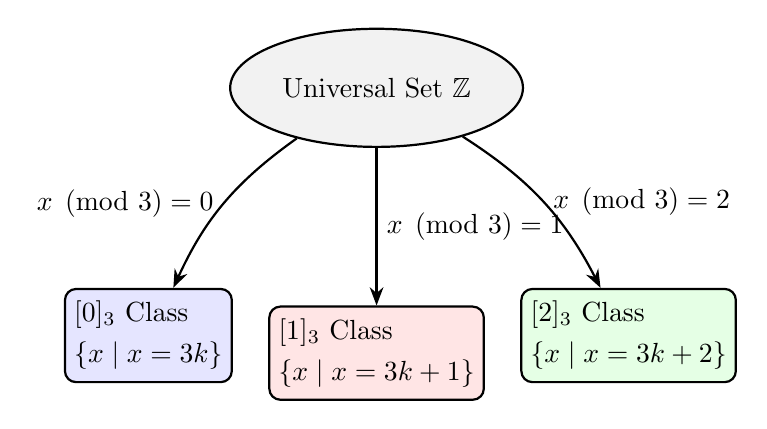
\begin{tikzpicture}[>=Stealth, node distance=1.5cm and 2cm, auto, thick]
  % Nodes
  \node[draw, ellipse, minimum width=3cm, minimum height=1.5cm, fill=gray!10] (Z) {Universal Set $\mathbb{Z}$};
  
  \node[draw, rectangle, rounded corners, fill=blue!10, below left=2cm and 0.5cm of Z] (C0) {
    $\begin{aligned}
    &[0]_3 \text{ Class} \\
    &\{x \mid x = 3k\}
    \end{aligned}$
  };
  
  \node[draw, rectangle, rounded corners, fill=red!10, below=2cm of Z] (C1) {
    $\begin{aligned}
    &[1]_3 \text{ Class} \\
    &\{x \mid x = 3k+1\}
    \end{aligned}$
  };
  
  \node[draw, rectangle, rounded corners, fill=green!10, below right=2cm and 0.5cm of Z] (C2) {
    $\begin{aligned}
    &[2]_3 \text{ Class} \\
    &\{x \mid x = 3k+2\}
    \end{aligned}$
  };

  % Arrows
  \draw[->, bend right=15] (Z) to node[midway, left] {$x \pmod 3 = 0$} (C0);
  \draw[->] (Z) to node[midway, right] {$x \pmod 3 = 1$} (C1);
  \draw[->, bend left=15] (Z) to node[midway, right] {$x \pmod 3 = 2$} (C2);
\end{tikzpicture}
\end{center}

\subsection{Heuristics \& "Cheats"}
\begin{itemize}
    \item \textbf{The "Not" Trigger:} If a problem asks you to prove a statement containing "does not divide" ($\nmid$), default immediately to setting up a Proof by Contrapositive. 
    \item \textbf{The Square Trigger:} If the problem involves proving divisibility properties of squares (e.g., $x^2, y^2$), modulo arithmetic (specifically modulo 3 or 4) is highly effective because the universe of possible remainders shrinks (e.g., $x^2 \pmod 4 \in \{0,1\}$).
\end{itemize}

\subsection{Pitfalls \& Fallacies}
\begin{itemize}
    \item \textbf{Assuming Prime Properties for Composites:} It is a fallacy to assume that if $a \mid bc$, then $a \mid b$ or $a \mid c$. This is \textit{only} true if $a$ is a prime number (Euclid's Lemma). Example of failure: $6 \mid (3 \times 4)$, but $6 \nmid 3$ and $6 \nmid 4$.
    \item \textbf{Dividing by Zero:} Writing $b/a$ instead of $b=ac$ often leads students to carelessly divide by variables that could be zero. Stick strictly to the multiplicative definition.
    \item \textbf{Circular Reasoning:} Assuming what you are trying to prove, often hidden within algebraic manipulation (e.g., factoring out the very integer you are trying to prove exists without defining it formally).
\end{itemize}

\newpage
% ---------------------------------------------------------
% PART 5: Conceptual Synthesis and The "Big Picture"
% ---------------------------------------------------------
\section{Part 5: Conceptual Synthesis and The ``Big Picture''}

\subsection{A) Thematic Connections}
The core theme of this chapter is \textit{structuring mathematical spaces via equivalence relations}. By declaring that $a$ relates to $b$ if $n \mid (a - b)$ (which we write as $a \equiv b \pmod n$), we collapse the infinite set of integers into finite, cyclic sets (e.g., $\mathbb{Z}_n$). This unifies previous topics of basic logic and algebraic manipulation into a rigorous, set-theoretic construction. Instead of viewing $1$ and $4$ as merely different numbers, under a modulo-3 framework, they become identical abstract entities residing in the same equivalence class $[1]_3$.

\subsection{B) Forward and Backward Links}
Backward, this chapter leans heavily on the algebraic closure of integers—the guarantee that the sum and product of integers remains an integer. Forward, these concepts form the necessary foundation for Abstract Algebra (Group, Ring, and Field theory). Specifically, understanding divisibility as forming ``ideals'' ($n\mathbb{Z}$) is a prerequisite to understanding Quotient Rings ($\mathbb{Z}/n\mathbb{Z}$). Ultimately, constructing fields like $\mathbb{Z}_p$ (where $p$ is prime) serves as the basis for probability theory over discrete, finite spaces, crucial for modern cryptanalysis and coding theory.

% ---------------------------------------------------------
% PART 6: Abstract Real-World Modeling (AI, ML, & Quant Finance)
% ---------------------------------------------------------
\section{Part 6: Abstract Real-World Modeling (AI, ML, \& Quant Finance)}

\subsection{A) Concrete Scenarios}
In quantitative finance and ML, abstract integer divisibility governs the foundational mechanisms of stochastic modeling.
\begin{enumerate}
    \item \textbf{Stochastic Simulation \& Random Number Generation:} Complex derivative pricing relies on Monte Carlo simulations, which require massive sets of uniform random numbers. These numbers are generated deterministically by Linear Congruential Generators (LCGs), which map state spaces over equivalence classes. The period of these generators dictates their usefulness, governed entirely by divisibility and prime factor properties (the Hull-Dobell Theorem).
    \item \textbf{Secure Multiparty Computation (Quant Trading):} Dark pools and decentralized trading protocols often use secret sharing schemes based on finite fields ($\mathbb{Z}_p$). Dividing assets/information into cryptographic shares requires precise properties of integer divisibility to ensure that the composite matrices used in these spaces remain invertible.
\end{enumerate}

\subsection{B) Model Problem Setup: Pseudo-Random SDE Discretization}
Suppose a quantitative researcher needs to price an exotic path-dependent Asian Option using a Black-Scholes framework. They must simulate the underlying asset's Geometric Brownian Motion (GBM). 

\textbf{1. The Underlying SDE:}
The stochastic differential equation under the risk-neutral measure $\mathbb{Q}$ is:
\[ dS_t = r S_t \, dt + \sigma S_t \, dW_t \]
where $W_t$ is a standard Brownian motion. To simulate paths via the Euler-Maruyama method over discrete time intervals $\Delta t$, we approximate increments as $\Delta W = \sqrt{\Delta t} Z$, where $Z \sim \mathcal{N}(0,1)$.

\textbf{2. The State Space and Divisibility Rules:}
To generate $Z$, we map a discrete integer state space to a uniform continuous space. We define a probability space $(\Omega, \mathcal{F}, \mathbb{P})$ relying on an LCG mapping over $\mathbb{Z}_M$.
Define a state sequence $X_n \in \{0, 1, \dots, M-1\}$ such that:
\[ X_{n+1} = (aX_n + c) \pmod M \]
To ensure the maximum sequence length (preventing the Monte Carlo from repeating paths and causing severe variance biases), we must satisfy the \textbf{Hull-Dobell Theorem}:
\begin{itemize}
    \item $c$ and $M$ are relatively prime (i.e., $\gcd(c, M) = 1$).
    \item For every prime divisor $p \mid M$, we must have $p \mid (a - 1)$.
    \item If $4 \mid M$, then $4 \mid (a - 1)$.
\end{itemize}

\textbf{3. Continuous Mapping (The SDE Bridge):}
Once a valid state sequence is generated, we map it to independent uniform variables $U_n = \frac{X_n}{M} \sim \text{Unif}(0,1)$.
Using the Box-Muller transform, we establish the standard normal mappings:
\[ Z_1 = \sqrt{-2\ln(U_1)} \cos(2\pi U_2) \]
We substitute this into our asset diffusion model:
\[ S_{t+\Delta t} = S_t \exp\left( \left(r - \frac{1}{2}\sigma^2\right)\Delta t + \sigma \sqrt{\Delta t} Z_1 \right) \]
Thus, the rigor of divisibility and prime factorization directly bounds the algorithmic integrity of trillion-dollar derivative pricing engines. If the mathematical parameters $a, c, M$ violate the strict abstract divisibility conditions, the state space collapses early, destroying the theoretical convergence of the Monte Carlo integral measure.

\newpage
% ---------------------------------------------------------
% PART 7: Common Variations and Untested Concepts
% ---------------------------------------------------------
\section{Part 7: Common Variations and Untested Concepts}

An essential theorem commonly tested in abstract mathematics, but missing from this specific homework slice, is \textbf{Euclid's Lemma} regarding prime numbers.

\begin{theorem}[Euclid's Lemma]
If $p$ is a prime number and $p \mid ab$, where $a, b \in \mathbb{Z}$, then $p \mid a$ or $p \mid b$.
\end{theorem}

\begin{proof}
Assume $p$ is prime and $p \mid ab$. Suppose for the sake of contraposition (or cases) that $p \nmid a$. Because $p$ is prime, its only divisors are $1$ and $p$. Since $p \nmid a$, the greatest common divisor of $p$ and $a$ must be $1$; they are relatively prime.
By B\'{e}zout's Identity, there exist integers $x, y \in \mathbb{Z}$ such that:
\[ px + ay = 1 \]
Multiply the entire equation by $b$:
\[ pbx + aby = b \]
We analyze the terms on the left:
1. $p(bx)$ is clearly a multiple of $p$, thus $p \mid pbx$.
2. We were given that $p \mid ab$, which means $ab = pk$ for some integer $k$. Substituting this, the second term is $pky$, which is a multiple of $p$.
Thus, the left side can be rewritten as:
\[ p(bx) + p(ky) = p(bx + ky) \]
Since $bx + ky$ is an integer, this demonstrates that $p$ divides the left side of the equation. Consequently, $p$ must divide the right side, which is $b$. Thus, $p \mid b$.
We have shown that if $p \mid ab$ and $p \nmid a$, then $p \mid b$. Therefore, $p \mid a$ or $p \mid b$.
\end{proof}

\vspace{2em}

% ---------------------------------------------------------
% PART 8: Advanced Diagnostic Testing: "Find the Flaw"
% ---------------------------------------------------------
\section{Part 8: Advanced Diagnostic Testing: ``Find the Flaw''}
\textit{Below are five flawed proofs. Your task is to act as a grader, identify the logical or mathematical error, and provide the correct reasoning.}

\subsection{Test Problems}

\textbf{Problem 1:} Let $a, b \in \mathbb{Z}$. Prove that if $4 \mid a^2$, then $4 \mid a$.
\begin{proof}[Flawed Proof 1]
Assume $4 \mid a^2$. By the definition of divisibility, $a^2 = 4k$ for some integer $k \in \mathbb{Z}$.
Taking the square root of both sides, we get $a = 2\sqrt{k}$.
Since $4 \mid a^2$, $a$ must be an even integer. Therefore, $a = 2m$ for some integer $m$. 
Since $a^2 = (2m)^2 = 4m^2$, and $4m^2$ is divisible by $4$, it must naturally follow that $a = 4q$ for some integer $q$, meaning $4 \mid a$.
\end{proof}

\textbf{Problem 2:} Let $a, b, c \in \mathbb{Z}$. Prove that if $a \mid b$ and $b \mid c$, then $b \mid a$.
\begin{proof}[Flawed Proof 2]
Assume $a \mid b$ and $b \mid c$. By definition, $b = ax$ and $c = by$ for some $x, y \in \mathbb{Z}$.
Substituting the first equation into the second, we get $c = (ax)y = a(xy)$.
Because integers are closed under multiplication, let $z = xy$. Then $c = az$.
By definition, this implies $a \mid c$. Since $a \mid c$ and $b \mid c$, it follows structurally that the divisors map onto each other symmetrically, meaning $b \mid a$.
\end{proof}

\textbf{Problem 3:} Let $n \in \mathbb{Z}$. Prove that if $n$ is not a multiple of 3, then $n^2 \equiv 1 \pmod 3$.
\begin{proof}[Flawed Proof 3]
Assume $n$ is not a multiple of 3. Then by the Division Algorithm, there is only one other possible remainder when avoiding strict multiples, meaning $n$ must take the form $n = 3k + 1$ for some integer $k$.
Squaring $n$, we obtain:
\[ n^2 = (3k + 1)^2 = 9k^2 + 6k + 1 = 3(3k^2 + 2k) + 1 \]
Let $m = 3k^2 + 2k$. Since $m \in \mathbb{Z}$, $n^2 = 3m + 1$. Thus, $n^2 \equiv 1 \pmod 3$.
\end{proof}

\textbf{Problem 4:} Prove that for any integer $x$, $0 \mid x \implies x = 0$.
\begin{proof}[Flawed Proof 4]
Assume $0 \mid x$. By definition, there exists an integer $k \in \mathbb{Z}$ such that $x = 0 \cdot k$.
Since any number multiplied by zero is zero, $x = 0$.
Furthermore, if we divide $x$ by 0, we see that $x/0 = k$. Since $k$ is defined as an integer, the expression is mathematically sound, reinforcing that $x$ is bound to 0. 
\end{proof}

\textbf{Problem 5:} Prove by contrapositive: If $a \nmid b$ and $a \nmid c$, then $a \nmid bc$.
\begin{proof}[Flawed Proof 5]
The statement is of the form $P \land Q \implies R$.
To prove this by contrapositive, we assume the negation of the conclusion, which is $\neg R$. Thus, assume $a \mid bc$.
We must show the negation of the hypothesis, which by De Morgan's Laws is $\neg (P \land Q) \equiv \neg P \land \neg Q$.
Therefore, we must show that $a \mid b$ and $a \mid c$.
Since $a \mid bc$, there exists an integer $k$ such that $bc = ak$. Let $k = xy$. Then $bc = axy$, which splits into $b = ax$ and $c = ay$. Thus $a \mid b$ and $a \mid c$, completing the contrapositive.
\end{proof}

\newpage
\subsection{Solution Key (For the Grader)}
\begin{itemize}
    \item \textbf{Resolution 1:} The flaw occurs when concluding ``it must naturally follow that $a = 4q$''. This is a non-sequitur jump. A counterexample is $a = 2$. $4 \mid 2^2$ (since $4 \mid 4$), but $4 \nmid 2$. The correct logic stops at $a$ being even ($2 \mid a$); $4 \mid a^2$ does not force $4 \mid a$.
    \item \textbf{Resolution 2:} The proof successfully shows $a \mid c$ (Transitive Property). The flaw is the arbitrary and entirely unfounded leap asserting ``divisors map onto each other symmetrically, meaning $b \mid a$''. Divisibility is a partial order, not a symmetric relation. Example: $2 \mid 4$ and $4 \mid 8$, but $4 \nmid 2$. 
    \item \textbf{Resolution 3:} The flaw is an incomplete application of the Division Algorithm (missing cases). The author assumes if $n \neq 3k$, then $n = 3k+1$. They completely forgot the third disjoint case: $n = 3k+2$. The proof must evaluate the $(3k+2)^2$ case as well (which also yields $3m+1$, saving the theorem, but the current proof is logically invalid).
    \item \textbf{Resolution 4:} The flaw is dividing by zero. The statement $x/0 = k$ is mathematically undefined and strictly prohibited in ring theory/real analysis. The proof was already complete at $x = 0 \cdot k = 0$. Dividing by zero introduces critical foundational violations.
    \item \textbf{Resolution 5:} The flaw is a misapplication of De Morgan's Laws. The negation of $(P \land Q)$ is $(\neg P \lor \neg Q)$, not $(\neg P \land \neg Q)$. The author attempts to prove "and", forcing an incorrect mathematical split. In reality, the proposition itself is false (e.g., let $a=6, b=2, c=3$. $6 \nmid 2$ and $6 \nmid 3$, but $6 \mid 6$). The contrapositive was incorrectly formulated, masking a false theorem.
\end{itemize}

\end{document}